%!TeX spellcheck = en-US
%!TEX root = ../hw1_report.tex
\subsection{(a)}
We compare GMRES and CGN for a given matrix $B$ and right hand side $b$. The result of the comparison is visualised in Figure \ref{task6}.
\begin{figure}[h!]
	\centering
	\begin{subfigure}[t]{0.49\textwidth}
		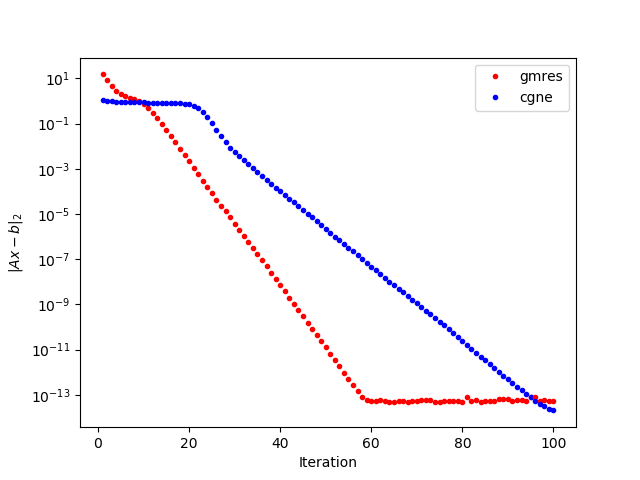
\includegraphics[width=\textwidth]{error_itr.png}
		\caption{Error versus number of iterations required for gmres and cgn for the given system.}
	\end{subfigure}~
	\begin{subfigure}[t]{0.49\textwidth}
		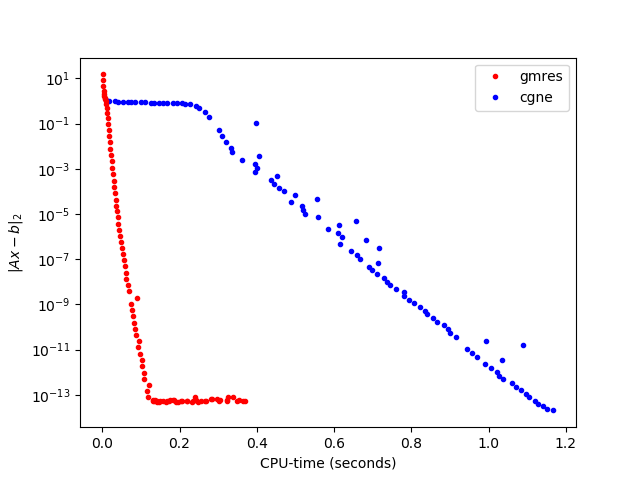
\includegraphics[width=\textwidth]{error_time.png}	
		\caption{Error versus CPU-time required for gmres and cgn for the given system.}
	\end{subfigure}
	\caption{}
	\label{task6}
\end{figure}
The iterates of CGN span a different Krylov subspace than gmres and it is mentioned in the lecture notes on this topic that in most cases, this subspace has worse approximation properties than the usual Krylov subspace used for the gmres iterates. This correspond with what can be observed in Figure \ref{task6}a. 
\subsection{(b)}
The result can be related to the convergence theory for CGN and GMRES.
